\chapter{Impact of misclassification and imperfect serological tests in association analyses of ME/CFS applied to Covid-19 data}
\label{chapter:misdiagnosis-serology-2022}
\chaptermark{Impact of misclassification and imperfect serological\\tests in association analyses of ME/CFS applied to Covid-19 data}



%%%%%%%%%%%%%%%%%%%%%%%%%%%%%%%%%%%%%%%%%%%%%%%%%%%%%%%%%%%%%%%%%%%%%%%%
\noindent\underline{J. Malato}, L. Graça, and N. Sepúlveda. Impact of misclassification and imperfect serological tests in association analyses of \cfs applied to COVID-19 data. In R. Bispo, L. Henriques-Rodrigues, R. Alpizar-Jara, and M. de Carvalho, editors, \textit{Recent Developments in Statistics and Data Science}, Springer Proceedings in Mathematics \& Statistics, pages 215--225, Cham, 2022. Springer International Publishing. ISBN 978-3-031-12766-3. doi: 10.1007/978-3-031-12766-315.

%%%%%%%%%%%%%%%%%%%%%%%%%%%%%%%%%%%%%%%%%%%%%%%%%%%%%%%%%%%%%%%%%%%%%%%%
\begin{abstract}
The diagnosis of \cfs is problematic due to the absence of a disease specific biomarker.
As such, it is conducted under uncertainty using symptom-based criteria and the exclusion of known diseases.
The possibility of misdiagnosing patients reduces the power to detect new and previously identified factors that can be associated with the disease.
To investigate this problem, we previously conducted a simulation study to estimate the power of case-control association studies as a function of the misdiagnosed rate.
Here we extended this simulation study to the more general situation where there is also the possibility of having misclassification in a binary factor related to a previous exposure to a given infection.
Given the suggested link between \cfs and past viral infections including SARS-CoV-2 (that causes Covid-19), we performed the simulation study in the specific context of serological testing of this new coronavirus using published data from Portuguese, Spanish and Iranian seroepidemiological studies.
\keywords{misclassification; simulation; power studies; serology; myalgic encephalomyelitis/chronic fatigue.}
\end{abstract}

%%%%%%%%%%%%%%%%%%%%%%%%%%%%%%%%%%%%%%%%%%%%%%%%%%%%%%%%%%%%%%%%%%%%%%%%
%%%%%%%%%%%%%%%%%%%%%%%%%%%%%%%%%%%%%%%%%%%%%%%%%%%%%%%%%%%%%%%%%%%%%%%%
%%%%%%%%%%%%%%%%%%%%%%%%%%%%%%%%%%%%%%%%%%%%%%%%%%%%%%%%%%%%%%%%%%%%%%%%
\section{Introduction}

Myalgic encephalomyelitis/Chronic fatigue syndrome (ME/CFS) is one example of a complex disease with uncertainty in its diagnosis \citep{nacul2017DifferingCase}. Patients diagnosed with this debilitating disorder manifest heterogeneous symptoms such as unexplained long-lasting fatigue \citep{fukuda1994ChronicFatigue}, post-exertional malaise that arises after slight physical, or mental effort and is not alleviated by rest \citep{carruthers2003MyalgicEncephalomyelitis}, accompanied by other symptoms. Its prevalence is estimated between 0.4\% and 1\% depending on the population, affecting more women than men, at a 6:1 ratio \citep{morrisMyalgicEncephalomyelitisChronic2013, lim2020SystematicReviewa}.

The aetiology of \cfs has been proved difficult to determine. Different reported factors such as acute infections, genetic predisposition, or environmental stressors can serve as triggers for the disease onset \citep{lacerdaLogisticRegressionAnalysis2019, chu2019OnsetPatterns}. Moreover there is no biomarker, or combination of biomarkers, that characterise this heterogeneous disease, which ultimately leave its diagnosis to be mostly done on the basis of specific symptoms and exclusion of other diseases \citep{smith2014DiagnosisTreatment}. This further increases the uncertainty surrounding an objective diagnosis, which has resulted in more than 20 symptom-based criteria currently used to clinically diagnose \cfs \citep{brurberg2014CaseDefinitions}. Despite proposed protocols for criteria standardisation in \cfs research \citep{pheby2020DevelopmentConsistent}, distinct studies will inevitably define the cohort of patients differently, potentially with conflicting results \citep{nacul2017DifferingCase}. This inherent level of mis\-clas\-sification---non-\cfs patients being incorrectly diagnosed as such---amongst \cfs cohorts has already been described in a study characterising the genome of suspected patients \citep{brown2021MECFS} and should be taken into account in order to minimise the negative effects on association studies \citep{malato2021Statisticalchallenges}.

Despite the pathomechanisms of \cfs remaining unknown, the disease has been described as having an autoimmune onset \citep{lorussoImmunologicalAspectsChronic2009, sotznyMyalgicEncephalomyelitisChronic2018}. This immune dysregulation often occurs after exposure to an acute viral infection \citep{rasa2018ChronicViral, blomberg2018InfectionEliciteda, chu2019OnsetPatterns}, with multiple association studies relating the exposure to viruses as trigger for \cfs development \citep{bansalChronicFatigueSyndrome2012, sotznyMyalgicEncephalomyelitisChronic2018}. Serological surveys have thus been conducted to better understand the role of distinct viruses in this disease. However, so far there have not been replicable confirmed associations. Possible arguments for this can be the disparate cohorts of (inherently misclassified) suspected \cfs patients used and other factors related to study design such as the low sample sizes used \citep{scheibenbogen2017EuropeanME} or the further stratification of patients into different subtypes \citep{jason2005ChronicFatigue}. Additionally, the serological tests used to assess exposure/non-exposure to the viruses are based on predetermined and arbitrary cutoff values to determine seropositive individuals \citep{scheibenbogen2017EuropeanME}. This important but often overlooked aspect can potentially add an additional layer to the misclassification on \cfs, with impacts on the studies' reproducibility \citep{domingues2021HerpesvirusesSerologya}.

Previously, we studied the dissimilarity between different symptom diagnosis criteria and simulated the impacts of misclassification in a single scenario of potential misdiagnosis of suspected patients \citep{malato2021Statisticalchallenges}. In the present paper we extended the proposed ideas on misclassification and studied its impact on the statistical power of serology hypothetical association studies. More recently, studies have related \cfs and the chronic post-viral syndrome developed after infection by the SARS-CoV-2 virus, responsible for the Covid-19 pandemic \citep{komaroffWillCOVID19Lead2021}. Despite the need for more extensive research on this topic, studies have reported that subset of patients following Covid-19 infection can develop a chronic syndrome that fulfils \cfs diagnostic criteria \citep{kedorChronicCOVID19Syndrome2021}. For illustrative purposes we extrapolated on the idea that there is in fact an association between Covid-19 and \cfs onset, however mild ($1.25 \leq \text{odds ratio} \leq 2.0$), and simulated multiple case-control association studies with different sample sizes, using results for seroprevalence surveys from three countries: Portugal \citep{kislayaSeroprevalenceSARSCoV2Infection2021}, Spain \citep{pollanPrevalenceSARSCoV2Spain2020}, and Iran \citep{khalagiPrevalenceCOVID19Iran2021}. For each serology study, we hypothesised on the impact of misclassification, also accounting for the estimated levels of sensitivity and specificity.

%%%%%%%%%%%%%%%%%%%%%%%%%%%%%%%%%%%%%%%%%%%%%%%%%%%%%%%%%%%%%%%%%%%%%%%%
%%%%%%%%%%%%%%%%%%%%%%%%%%%%%%%%%%%%%%%%%%%%%%%%%%%%%%%%%%%%%%%%%%%%%%%%
%%%%%%%%%%%%%%%%%%%%%%%%%%%%%%%%%%%%%%%%%%%%%%%%%%%%%%%%%%%%%%%%%%%%%%%%
\section{Simulation study}

%%%%%%%%%%%%%%%%%%%%%%%%%%%%%%%%%%%%%%%%%%%%%%%%%%%%%%%%%%%%%%%%%%%%%%%%
\subsection{Mathematical formulation of the problem}

Following-up on the reported ideas on misclassification \citep{malato2021Statisticalchallenges}, the goal of the proposed hypothetical study was to assess the association of a binary exposure outcome (as exposed versus non-exposed) after a serological survey for Covid-19 with \cfs. This was accomplished by comparing a cohort of sampled patients suspected of \cfs to a cohort of sampled matched healthy controls. The sampling distribution of the designed case-control study was then, the product of two Binomial distributions given by the number of sampled individuals from the two cohorts, $n_0$ and $n_1$, respectively for healthy controls and suspected \cfs patients, and the probability of exposure to the virus, $\theta_0$ and $\theta_1$, respectively; with $x_0$ and $x_1$ being the observed frequencies of exposed healthy controls and suspected \cfs \citep{malato2021Statisticalchallenges}. Altogether, the sampled populations can be summarised by a $2 \times 2$ frequency table that presents different outlines depending on the described parameters $n_i$ and $\theta_i$, $i = \{0,1\}$. Testing the null hypothesis for lack of association to \cfs (i.e., $H_0: \theta_0 = \theta_1$) was done through the Pearson's $\chi^2$ test for independence. After testing, $H_0$ was rejected if the p-value for the Pearson's $\chi^2$ test was less than the prespecified level of significance of 5\%. Through simulation, and by repeating the inference multiple times under the same conditions, the power of the study was estimated as the overall proportion in which $H_0$ was rejected.

Previously \citep{malato2021Statisticalchallenges}, to account for the inherent misclassification as a diluting effect for the detection of a potential association, four assumptions were considered for the \cfs cohort: (i) sampled suspected \cfs cases can be divided into apparent (false positives) and true positive cases; (ii) the misclassified apparent cases are considered healthy controls, in the sense that they share the same probability of exposure to Covid-19, $\theta_0$; (iii) there is an overall misclassification rate, $\gamma$, creating the two distinct possibilities of apparent and true cases within the cohort for suspected cases; and (iv) this misclassification rate is only dependent on the true clinical status of each of the suspected cases. Under the assumption (ii) and the law of total probability, the probability of exposure associated with the suspected cases was written as
% 
\begin{equation}
    \theta_1 = \gamma \theta_0 + (1 - \gamma) \theta_{1}^{*}\ ,
    \label{eq:theta_11}
\end{equation}
% Equation (1)
% Equation~(\ref{eq:theta_11})
% 
where $\theta_{1}^{*}$ is the exposure probability of true \cfs cases.

However, this analysis does not account for the sensitivity and specificity of a serology test if the exposure to a given infection is determined this way. Therefore, four additional assumptions were considered for this study, with effects transversal to all data sets: (v) for each serology test performed, individuals can only be classified as seropositive or seronegative---in opposition to serology tests where there are more than two possible outcomes; (vi) the levels of sensitivity, $\pi_{se}$, and specificity, $\pi_{sp}$, respectively determine the accuracy of a test to identify truly exposed and truly non-exposed individuals; (vii) these parameters related to the performance of the serology test create a category of undetected false positives and false negative for individuals poorly measured by the serology assessment; and (viii) the binary exposure outcomes given by $\pi_{se}$ and $\pi_{sp}$ are independent from the assessed cohort. Under these assumptions, the probability of exposure for suspected cases from Equation~(\ref{eq:theta_11}) can be extended to
% 
\begin{equation}
    \theta_{1} = \pi_{se}\gamma\theta_{0} + (1-\pi_{sp})\gamma(1-\theta_{0}) + \pi_{se}(1-\gamma)\theta_{1}^* + (1-\pi_{sp})(1-\gamma)(1-\theta_{1}^*)\ .
    \label{eq:theta_12}
\end{equation}
% Equation (2)
% Equation~(\ref{eq:theta_12})
% 
Under the eight assumptions, the observable $2 \times 2$ frequency table can be augmented, as the cohort for suspected \cfs is divided into apparent and true cases based on the misclassification rate, $\gamma$, and with sensitivity and specificity, respectively $\pi_{se}$ and $\pi_{sp}$, defining the serology tests' overall accuracy to determine the seropositive (either true positive or false positive) and seronegative (both true and false negative) populations on both cohorts (Table~\ref{tab:seroprobs})\footnote{Instead of the Pearson's $\chi^2$ test, an analogous investigation could also been proposed using the Fisher's exact test to assess the null hypothesis for lack of association. Equation~(\ref{eq:theta_12}) includes parameters related to the accuracy of serology tests; based on this formulation, one can obtain Equation~(\ref{eq:theta_11}) by simply assuming $\pi_{se} = \pi_{sp} = 1$.}.

\begin{table}
    \centering
    \caption[Augmented version of the observable $2 \times 2$ frequency table in the case-control association study scenario with possible misclassification of suspected \cfs cases and existence of false positive and false negative serological outcomes observed from serology tests done to assess exposure]{Augmented version of the observable $2 \times 2$ frequency table in the case-control association study scenario with possible misclassification of suspected \cfs cases (into apparent and true cases) and existence of false positive and false negative serological outcomes observed from serology tests done to assess exposure (confirmed by the true exposure indicator columns, with $E$ for exposed individuals and $\overline{E}$ for non-exposed).}
    \resizebox{\textwidth}{!}{\begin{tabular}{lcccc} 
\toprule
\multirow{2}{*}{\begin{tabular}[c]{@{}c@{}}Observed \\test outcome\end{tabular}} & \multirow{2}{*}{\begin{tabular}[c]{@{}c@{}}True exposure \\indicator\end{tabular}} & \multirow{2}{*}{Controls}  & \multicolumn{2}{c}{Suspected cases} \\ 
\cline{4-5}
                                                                                 &                &                            & (Apparent)                       & (True)                                \\ 
\hline
\multirow{2}{*}{Seropositive}                                                    & $E$            & $\pi_{se}\theta_0$         & $\pi_{se}\gamma\theta_0$         & $\pi_{se}(1-\gamma)\theta_1^*$        \\
                                                                                 & $\overline{E}$ & $(1-\pi_{sp})(1-\theta_0)$ & $(1-\pi_{sp})\gamma(1-\theta_0)$ & $(1-\pi_{sp})(1-\gamma)(1-\theta_1^*)$ \\
\cmidrule{2-5}
\multirow{2}{*}{Seronegative}                                                    & $E$            & $(1-\pi_{se})\theta_0$     & $(1-\pi_{se})\gamma\theta_0$     & $(1-\pi_{se})(1-\gamma)\theta_1^*$    \\
                                                                                 & $\overline{E}$ & $\pi_{sp}(1-\theta_0)$     & $\pi_{sp}\gamma(1-\theta_0)$     & $\pi_{sp}(1-\gamma)(1-\theta_1^*)$    \\
\bottomrule
\end{tabular}
}
    \label{tab:seroprobs}
\end{table}
% Table 1
% Table~\ref{tab:seroprobs}

%%%%%%%%%%%%%%%%%%%%%%%%%%%%%%%%%%%%%%%%%%%%%%%%%%%%%%%%%%%%%%%%%%%%%%%%
\subsection{Parameterisation using real-word data}

As example of real-life application, we looked at data from three distinct seroepidemiologic surveys: Portugal \citep{kislayaSeroprevalenceSARSCoV2Infection2021}, Spain \citep{pollanPrevalenceSARSCoV2Spain2020}, and Iran \citep{khalagiPrevalenceCOVID19Iran2021}. The studies occurred between April and August 2020 and applied similar methods of estimation of their populations' seroprevalence. Also, all surveys presented information regarding the sensitivity and specificity estimates for the serology tests performed. The estimated values for the mentioned parameters in each survey are presented in Table~\ref{tab:paper-parameters}.

\begin{table}[h]
    \centering
    \caption[Parameter values used in the study]{Parameter values used in the study, where the probability of exposure to the virus and the sensitivity and specificity of the serology test are given by $\theta_0$, $\pi_{se}$, and $\pi_{sp}$, respectively.}
    \begin{tabular}{llcccccc} 
\toprule
Reference & Country &  & $\theta_0$ &  & $\pi_{se}$ &  & $\pi_{sp}$ \\ 
\midrule
\citet{kislayaSeroprevalenceSARSCoV2Infection2021} & Portugal & & 0.025 & & 0.95 & & 0.98 \\
\citet{pollanPrevalenceSARSCoV2Spain2020}  & Spain    & & 0.050 & & 0.80 & & 0.98 \\
\citet{khalagiPrevalenceCOVID19Iran2021} & Iran     & & 0.150 & & 0.75 & & 0.98 \\
\bottomrule
\end{tabular}
    \label{tab:paper-parameters}
\end{table}
% Table 2
% Table~\ref{tab:paper-parameters}

For the purpose of the study, we assumed the existence of an association between exposure to Covid-19 and \cfs onset. Despite few evidences thus far due to the novelty of the topic, some studies have mentioned this association based on the idea of immune dysregulation, linking the development of post-Covid-19 chronic symptoms with the autoimmune proposal for \cfs \citep{sotznyMyalgicEncephalomyelitisChronic2018}. Since there are no biomarkers for \cfs diagnosis, we defined the association as a mild relation with three possible values of the overall true odds ratio, $\Delta_T = \{1.25, 1.5, 2\}$. Based on the values of $\theta_0$ from the three surveys and the proposed $\Delta_T$, the probability of exposure on true \cfs cases was determined by
% 
\begin{equation}
    \theta_1^* = \frac{\theta_0\Delta_T}{1 + \theta_0 \left(\Delta_T - 1\right)}\ .
    \label{eq:or_t}
\end{equation}
% Equation (3)
% Equation~(\ref{eq:or_t})

%%%%%%%%%%%%%%%%%%%%%%%%%%%%%%%%%%%%%%%%%%%%%%%%%%%%%%%%%%%%%%%%%%%%%%%%
\subsection{Simulation structure}

The impact of inherent misclassification on the hypothetical case-control association studies was assessed through multiple simulations on different parametric values for $\theta_0$, $\pi_{se}$, $\pi_{sp}$, in accordance to each serological survey (Table~\ref{tab:paper-parameters}), and $\Delta_T$. For each combination of $\theta_0$ and $\Delta_T$, parameters $\theta_1$ and $\theta_1^*$ were calculated from Equation~(\ref{eq:theta_12}) and Equation~(\ref{eq:or_t}), respectively. To illustrate how sample sizes also influence the overall power of a study, we performed our simulations considering cohort sample sizes of $n_0 = n_1 = \{100, 250, 500, 1000, 2500, 5000\}$.

To assess the power of rejecting $H_0$, 10,000 data sets were generated for each value of $\gamma$, ranging from 0 (no misclassification) to 1 (no true \cfs patients in the cohort for suspected cases) with a lag of 0.01. As previously mentioned, $H_0$ was rejected at each data set if the p-value from the Pearson's $\chi^2$ test was less than the usual level of significance. Finally, for each parameter set, power was estimated as the proportion of simulated data sets in which $H_0$ was rejected.% with 95\% confidence intervals estimated using the Wald method.
All simulations and analyses were done using R statistical software, version 4.1.0 \citep{rcoreteamLanguageEnvironmentStatistical2020}, using our own scripts, available upon request\footnote{For the purpose of study consistency, the estimated seroprevalence values published on the serological surveys were considered as the probability of exposure in the cohort of matched healthy controls, $\theta_0$.}.

%%%%%%%%%%%%%%%%%%%%%%%%%%%%%%%%%%%%%%%%%%%%%%%%%%%%%%%%%%%%%%%%%%%%%%%%
%%%%%%%%%%%%%%%%%%%%%%%%%%%%%%%%%%%%%%%%%%%%%%%%%%%%%%%%%%%%%%%%%%%%%%%%
%%%%%%%%%%%%%%%%%%%%%%%%%%%%%%%%%%%%%%%%%%%%%%%%%%%%%%%%%%%%%%%%%%%%%%%%
\section{Simulation results}

As expected, the estimated power to detect the hypothetical association decreased with misclassification rate (Figure~\ref{fig:misrate-country}). Looking at the extreme cases, the estimated power was highest when no misclassification was considered and all suspected \cfs cases were considered to be true positives ($\gamma = 0$). Irrespective of the scenario, as misclassification increases, the overall power is reduced towards 5\% at the opposite most extreme value ($\gamma = 1$)---i.e., the significance level specified for the Pearson's $\chi^2$ test.

\begin{figure}
    \centering\resizebox{\linewidth}{!}{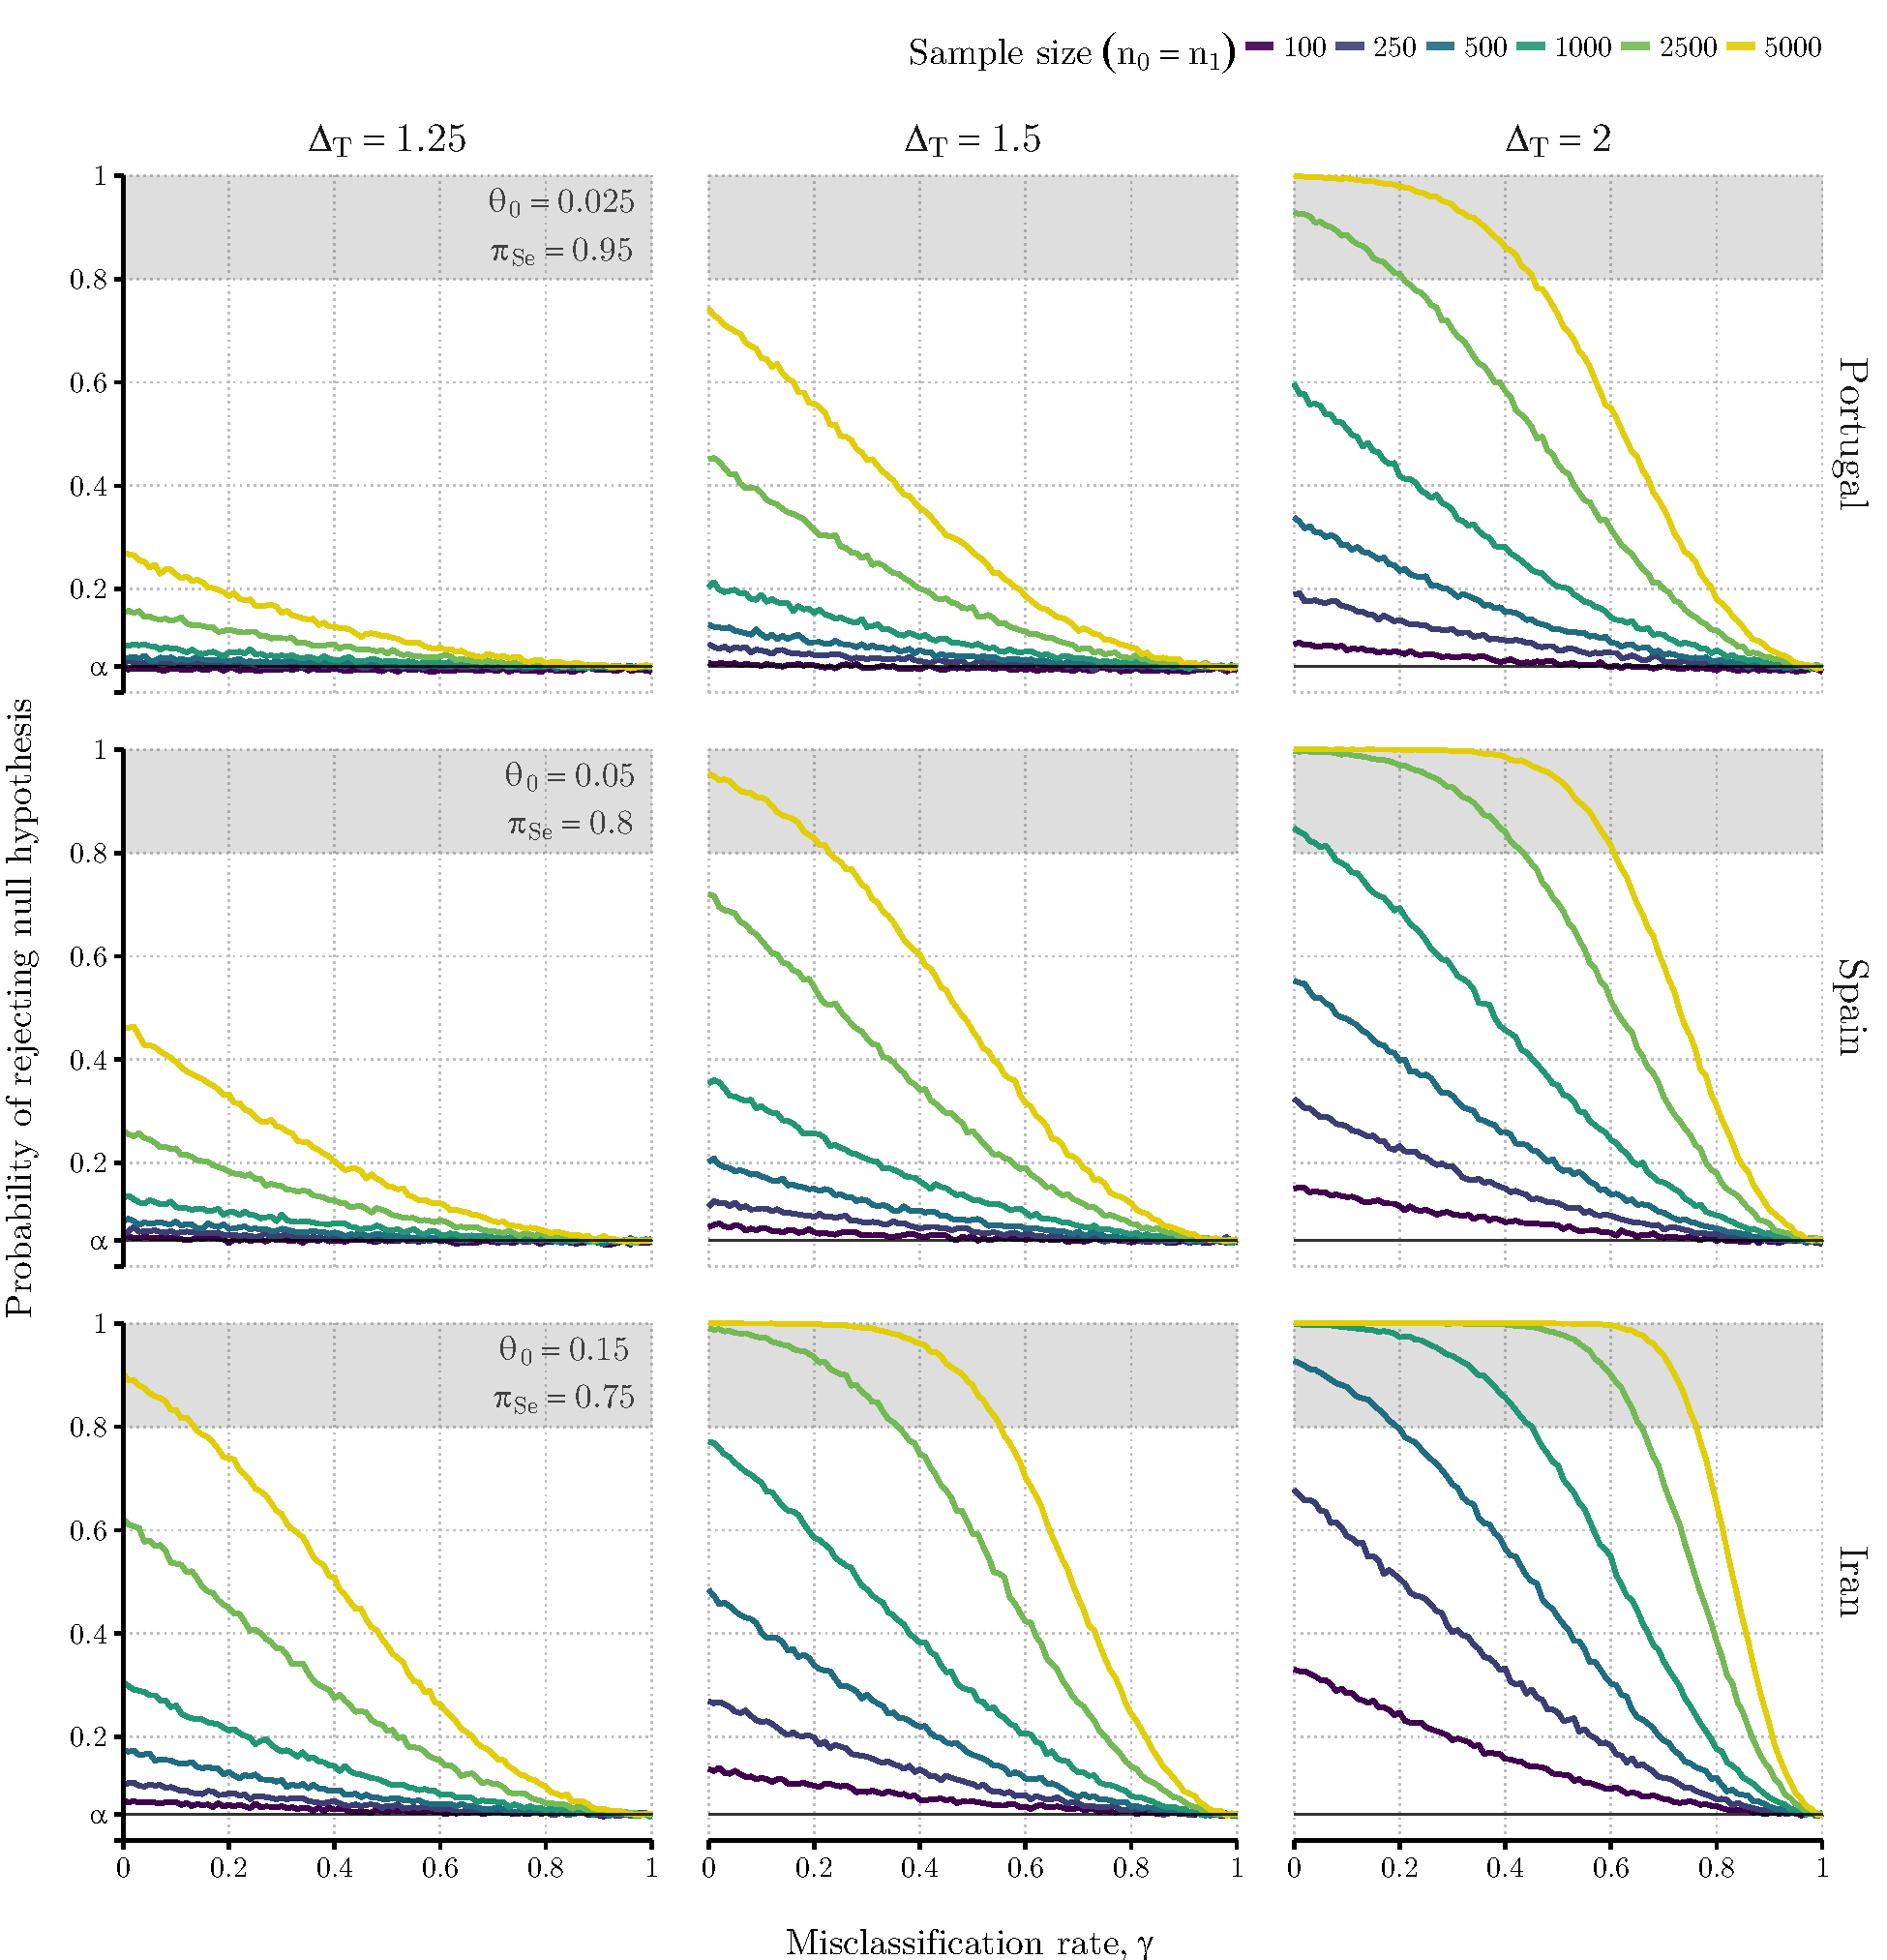
\includegraphics{chapter/2022-misdiagnosis-serology/figures/spe2021_012_fig1.pdf}}
    \caption[Probabilities of rejecting the null hypothesis as function of the misclassification rate]{Probabilities of rejecting the null hypothesis, i.e., absence of association between the two populations as function of the misclassification rate. Each column represents the values attributed to the true odds ratio for Covid-19 exposure and true \cfs, assessed between true positive cases and healthy controls. Each row indicates a country serologic survey, with distinct values of $\theta_0$ and $\pi_{se}$ identified in the first column of each survey, and fixed $\pi_{sp} = 0.98$ across all simulations. Power analysis was estimated for different cohort sample sizes of 100, 250, 500, 1000, 2500, and 5000 individuals ($n_0 = n_1$), represented by the lines of different colours in each scenario. Gray filled area indicates scenarios where the probability of rejecting the null hypothesis is above 80\%. Dark horizontal line indicates the level of significance used, $\alpha=0.05$.}
    \label{fig:misrate-country}
\end{figure}
% Figure 1
% Figure~\ref{fig:misrate-country}

Along with gradually increasing the misclassification of suspected patients, the power to detect an association was estimated by varying the values of probability of exposure in healthy controls, $\theta_0$, and sensitivity of the serology test, $\pi_{se}$, for each country serological scenario. In all three illustrated scenarios, the specificity was the same and estimated at $\pi_{sp}=0.98$ (Table~\ref{tab:paper-parameters}).

Overall, only sample sizes of $n_i \geq 500$ individuals were able to reach a power of at least 80\%---the specified power threshold to identify what can be considered as having acceptable reproducibility level (Table~\ref{tab:p80}). Simulations with larger sample sizes granted a consistency to the reproducibility of the studies, with power remaining above the defined threshold for higher values of misclassification. Similarly, higher values of $\Delta_T$ also affected positively the overall power of each study (Table~\ref{tab:p80}).

% PORTUGAL
The Portuguese survey had the smallest estimate for the probability of virus exposure and the highest sensitivity \citep{kislayaSeroprevalenceSARSCoV2Infection2021}. For this scenario, only higher association values of $\Delta_T = 2$ and cohort sample sizes of 2500 and 5000 reached the power of at least 80\%. Under these parametric conditions, the acceptable level of reproducibility was observable at $\gamma \leq 0.45$.

% SPAIN
Compared to Portugal's results, the Spain's survey had $\theta_0$ increased and the $\pi_{se}$ decreased \citep{pollanPrevalenceSARSCoV2Spain2020}. In this scenario there was an increase on the reproducibility, with more studies surpassing the 80\% threshold. Nonetheless, this only occurred for sample sizes of $n_i \geq 1000$.

% IRAN
Lastly, Iran's survey \citep{khalagiPrevalenceCOVID19Iran2021} had the highest estimate for $\theta_0$ and lowest estimates for $\pi_{se}$. Despite the lower sensitivity, simulations under these parameters had higher power for the same sample sizes than the other two scenarios (Figure~\ref{fig:misrate-country} and Table~\ref{tab:p80}).

\begin{table}[h]
    \centering
    \caption[Maximum values of misclassification rate that maintain power if at least 80\% to reject the null hypothesis of lack of association, for different values of true odds ratio country of serological survey, and sample sizes]{Maximum values of misclassification rate, $\gamma$, that maintain power if at least 80\% to reject the null hypothesis of lack of association, for different values of true odds ratio, $\Delta_T$, country of serological survey, and sample sizes, $n_{i}$, $i=(0, 1)$. Cells with no value indicate the inability to reach the power threshold between cohort, even at $\gamma = 0$.}
    \begin{tabular}{c!{\vrule width \lightrulewidth}ccc!{\vrule width \lightrulewidth}c} 
\toprule
\diagbox{Country}{$\Delta_T$} & 1.25 & 1.50 & 2.00 & $n_i$ \\
\midrule
Portugal   & $-$  & $-$  & $-$  & \multirow{3}{*}{100}  \\
Spain      & $-$  & $-$  & $-$  &                       \\
Iran       & $-$  & $-$  & $-$  &                       \\ 
\midrule
Portugal   & $-$  & $-$  & $-$  & \multirow{3}{*}{250}  \\
Spain      & $-$  & $-$  & $-$  &                       \\
Iran       & $-$  & $-$  & $-$  &                       \\ 
\midrule
Portugal   & $-$  & $-$  & $-$  & \multirow{3}{*}{500}  \\
Spain      & $-$  & $-$  & $-$  &                       \\
Iran       & $-$  & $-$  & 0.19 &                       \\ 
\midrule
Portugal   & $-$  & $-$  & $-$  & \multirow{3}{*}{1000} \\
Spain      & $-$  & $-$  & 0.07 &                       \\
Iran       & $-$  & $-$  & 0.45 &                       \\ 
\midrule
Portugal   & $-$  & $-$  & 0.20 & \multirow{3}{*}{2500} \\
Spain      & $-$  & $-$  & 0.43 &                       \\
Iran       & $-$  & 0.35 & 0.65 &                       \\ 
\midrule
Portugal   & $-$  & $-$  & 0.45 & \multirow{3}{*}{5000} \\
Spain      & $-$  & 0.22 & 0.60 &                       \\
Iran       & 0.13 & 0.55 & 0.76 &                       \\
\bottomrule
\end{tabular}
    \label{tab:p80}
\end{table}
% Table 3
% Table~\ref{tab:p80}

%%%%%%%%%%%%%%%%%%%%%%%%%%%%%%%%%%%%%%%%%%%%%%%%%%%%%%%%%%%%%%%%%%%%%%%%
%%%%%%%%%%%%%%%%%%%%%%%%%%%%%%%%%%%%%%%%%%%%%%%%%%%%%%%%%%%%%%%%%%%%%%%%
%%%%%%%%%%%%%%%%%%%%%%%%%%%%%%%%%%%%%%%%%%%%%%%%%%%%%%%%%%%%%%%%%%%%%%%%
\section{Discussion}

Focusing on \cfs, our simulation results showed how misclassification of patients poses an impact on the ability to consistently recognise true associations to a triggering viral exposure, prior to the disease onset. While still researching for biomarkers able discriminate the disease, the power is very likely to suffer from limited statistical power due to possible misclassification of the suspected \cfs cases. The proposed solution to this problem is to take into account for misclassification in the respective statistical analysis.

The results evidenced how increasing a study's sample size can increase its power. Until now, misclassification studies mostly focused on identifying the extent of misdiagnosed of patients when using distinct diagnosis criteria, not particularly looking at sample sizes \citep{malato2021Statisticalchallenges}. With \cfs research being usually underfunded \citep{dimmockEstimatingDiseaseBurden2016, mirinResearchUpdateRelation2020}, case-control studies are frequently performed on sample sizes below 250 patients. This allows for potential sporadic associations that ultimately cannot be replicated in follow-up studies. Throughout efforts to raise awareness and laboratory collaborations, studies have been increasing their sampled populations. After all, our study showed that under the parameterised conditions, only cohorts with samples above 500 individuals were able to consistently reject the null hypothesis under some levels of misclassification (Table~\ref{tab:p80}).

A more in depth study would be required to pose a more general conclusion on the influence in power caused by prevalence of exposure and the sensitivity and specificity of the serology test. One can argue that increasing the prevalence will make for better comparisons between cohorts through the Pearson's $\chi^2$ test for independence, as it might improve the frequency distributions across the $2 \times 2$ contingency table cells. Whereas, sensitivity and specificity will produce a lessened effect, as serology tests keep improving---but still impactful, if not from the estimated $\pi_{se}$ and $\pi_{sp}$, then because the majority of serological cutoff values for seropositivity used arise from inherently arbitrary choices if the researchers and manufacturers of the serology tests \citep{domingues2021HerpesvirusesSerologya, domingues2021AnalysisAntibody}. Nevertheless, diagnostic accuracy is still of extremely importance in the evaluation of medical diagnostic tests and should be taken into account when replication of a study---in this case, a scenario of a serology study---is necessary.

This hypothetical study was done in the context of the recent Covid-19 pandemic and the association of the long-term symptoms caused by the SARS-CoV-2 virus and \cfs diagnosis. With the lack of extensive information on this Covid-19 exposure-\cfs diagnosis relation premise, parameter $\Delta_T$ was defined within low-to-mild values as to not profoundly influence the simulation results. As more studies and serological surveys are published on the matter, focusing different populations or even focusing on serology tests for different specific antibodies against Covid-19, one could better parameterise the simulation study.

% Concluding remarks -------------------------------
\cfs is a complex disease and there is still lack of understanding to the extension of the disease's aetiology and pathophysiology. Even under these uncertainties, accepting and accounting for a level of patient misclassification---however small---in association studies might help to improve the study designs and increase scientific reproducibility. Ultimately, the ability to replicate and reproduce the results proposed by a study is one of the most important aspects in research, and consistent results are what allows ideas to become postulates, continuously driving science forwards.
% \vfill
% \newpage

%%%%%%%%%%%%%%%%%%%%%%%%%%%%%%%%%%%%%%%%%%%%%%%%%%%%%%%%%%%%%%%%%%%%%%%%
\addcontentsline{toc}{section}{Bibliography}
\bibliographystyle{abbrvnat}
\bibliography{references}
%%%%%%%%%%%%%%%%%%%%%%%%%%%%%%%%%%%%%%%%%%%%%%%%%%%%%%%%%%%%%%%%%%%%%%%%

% Equation (1)
% Equation~(\ref{eq:theta_11})
% Equation (2)
% Equation~(\ref{eq:theta_12})
% Equation (3)
% Equation~(\ref{eq:or_t})

% Table 1
% Table~\ref{tab:seroprobs}
% Table 2
% Table~\ref{tab:paper-parameters}
% Table 3
% Table~\ref{tab:p80}

% Figure 1
% Figure~\ref{fig:misrate-country}
